\documentclass[9pt,twocolumn,twoside]{g3_article/gsag3jnl}

% Packages.

\usepackage{multirow}
\usepackage{caption}

% Custom Commands.
\newcommand{\etal}{\textit{et al.}}

\articletype{gs} % article type
% {inv} Investigations
% {msr} Mutant Screen Reports
% {gs} Genomic Selection
% {goi} Genetics of Immunity 
% {gos} Genetics of Sex 
% {mp} Multiparental Populations

\title{Genomic Selection with Deep Neural Networks}

\author[$\ast$,1]{Riley McDowell}
\author[$\dagger$]{David Grant}
%\author[$\ddagger$]{Author Three}
%\author[$\S$]{Author Four}
%\author[$\ast\ast$]{Author Five}

\affil[$\ast$]{Iowa State University, US}
\affil[$\dagger$]{Iowa State University, US}
%\affil[$\ddagger$]{Author three affiliation}
%\affil[$\S$]{Author four affiliation}
%\affil[$\ast\ast$]{Author five affiliation}

%For the authors' names, indicate different affiliations with the 
%symbols: $\ast$, $\dagger$, $\ddagger$, $\S$. After four authors
%, the symbols double, triple, quadruple, and so forth as required.

\keywords{ genomic prediction \\ deep learning \\ neural network \\ genomic selection \\ SNP }

\runningtitle{ Genomic Selection with Deep Neural Networks } % Goes into the footer.

\correspondingauthor{Corresponding Author HERE} % TODO: Who is this?

\begin{abstract}

Reduced costs for DNA marker technology coupled has generated a huge amount of
molecular data and greatly increased the options available to characterize lines 
in a breeding program. Concurrently, the field of machine learning has experienced
a resurgence of research into techniques to detect or "learn" patterns in noisy
data in a variety of technical applications. Here, we apply so called "deep learning"
techniques from current machine learning research in neural networks to 
genomic selection and phenotypic selection problems on published reference datasets. 
We compare the results of these algorithms to the bayesian and linear regression techniques
commonly employed today.


%The abstract should be written for people who may not read the 
%entire paper, so it must stand on its own.  The impression it makes usually determines 
%whether the reader will go on to read the article, so the abstract must be 
%engaging, clear, and concise.  In addition, the abstract may be the only part of the 
%article that is indexed in databases, so it must accurately reflect the 
%content of the article. A well-written abstract is the  most effective way to reach intended 
%readers, leading to more robust search, retrieval, and usage of the article. 
%
%Please see additional guidelines notes on preparing your abstract below.

%\begin{itemize}
%\item provide a synopsis of the entire article;
%\item begin with the broad context of the study, followed by specific background for the study;
%\item describe the purpose, methods and procedures, core findings and results, and conclusions of the study;
%\item emphasize new or important aspects of the research;
%\item engage the broad readership of G3 and be understandable to a diverse audience (avoid using jargon);
%\item be a single paragraph of less than 250 words;
%\item contain the full name of the organism studied;
%\item NOT contain citations or abbreviations.
%\end{itemize}

\end{abstract}

\setboolean{displaycopyright}{true}

\begin{document}

\maketitle
\thispagestyle{firststyle}
\logomark
\articletypemark
\marginmark
\firstpagefootnote
\correspondingauthoraffiliation{CORRESPONDING AUTHOR ADDRESS AND EMAIL}
\vspace{-11pt}%

\noindent % Skip header for 'Introduction'.

Markers are useful because they can be associated with traits.
QTL mapping, most useful for traits with small number of contributing loci.
Not useful for early breeding program selection or phenotypic prediction.

Meuwissen et al. (2001) publishes paper on genomic selection using
simulated data demonstrating prediction of offspring performance
from genotypic data using mixed models and bayesian methods.
Bayesian methods are most accurate.

Technique is applied to animal breeding, then plant breeding,
both successfully. Several alternate methods used. 

Several articles publish data and genomic selection algorithms,
reporting the accuracy of each on the dataset. One includes 
simple artificial neural network.

Concurrently, artificial intelligence research is rebranded as machine
learning, and the popularity of the interdisciplinary field known as data science 
increases dramatically. Data scientists apply machine learning and statistics 
from a wide variety of domains including mathematics, physics, and 
computer science to non-scientific domains such as sales and marketing.

Neural networks began gaining popularity with the rise of computers capable of
running the complex calculations required to train them. The most
common training procedure is backpropagation, where output errors are attributed
to prior network layers, adjusted, and remaining errors propagated backward
until the input layer is reached \citep{rumelhart1986}. Many thousands of small 
adjustments are made on batches of data until the error in the output is 
minimized. In the late 80s, it was shown that that multi-layer feedforward 
neural networks were capable of approximating functions of arbitrary complexity to 
arbitrary accuracy \citep{hornik1989}. With the rise of artificial intelligence
rebranded as machine learning, neural networks again surged in popularity,
but with considerably more computational power available. Networks that were
previously too complex to train in time to publish a paper can now be trained in
a matter of hours on a modern computer processor or high performance graphics card. 

Because networks are universal approximators, networks with many
neurons have a tendency to fit individual datapoints too tightly 
in a process known as overfitting. In order to fit the model to the underlying
sigmal rather than noise, a process called regularization is employed. One method
of regularization is to penalize weights $w$ with very large values \citep{krogh1992}. 
Another is to remove neurons and their connections at random during each training
epoch, allowing subsets of the network to for independent units of learning al.la. ensemble learning methods.  
This allows neurons to adapt and build independenty operating units and prevents the entire
network from co-adapting and overfitting the training set \citep{srivastava2014}.

Today, networks and award-winning performance in many domains \citep{schmidhuber2015}.

Historically, very large neural networks can take many CPU-hours to optimize and 
train, limiting their application \citep{gonzalez-recio2014}. 
% Probably a great citation/paper out there about how GPU compute has revolutionized
% neural network training.
Advances in machine 
learning coupled with Moore's Law and the widespread availability of programmable 
Graphics Processing Units (GPUs) opens neural networks to many problems and 
domains that would not have been possible a few years earlier. 

% For the introduction, authors should be mindful of the broad readership of the journal. i
% The introduction should set the stage for the importance of the work to a generalist 
% reader and draw the reader in to the specific study. The scope and impact of the 
% work should be clearly stated.

Authors are encouraged to:

\begin{itemize}
\item cite the supporting literature completely rather than select a subset of citations;
\item provide important background citations, including relevant review papers (to help orient the non-specialist reader);
\item to cite similar work in other organisms.
\end{itemize}

\section*{Materials and Methods}

Five benchmark datasets of paired phenotypic and genotypic marker data were predicted 
using a collection of regression techniques. Benchmark species included three food crops, 
one forestry species, and one animal species. Benchmark traits include a variety of high and low
heritability traits with simple and complex genetic archetectures. Each dataset was divided
into 10 partitions by drawing entries without replacement and predicted with each
regression technique using ten-fold cross validation. The partitions of the data were 
held constant across all regression techniques to facilitate a fair comparision of the
prediction accuracy of each technique.

For statistical models with tunable hyperparameters, a grid-search of the parameter 
space was conducted and the parameters that produced maximum hold-out set accuracy 
were used in the final analysis. 

%Manuscripts submitted to G3 should contain a clear description of the experimental design in sufficient detail so that 
%the experimental analysis could be repeated by another scientist. If the level of detail necessary to explain the 
%protocol goes beyond two paragraphs, give a short description in the main body of the paper and prepare a detailed 
%description for supporting information.  For example, details would include indicating how many individuals were used, 
%and if applicable how individuals or groups were combined for analysis. If working with mutants indicate how 
%many independent mutants were isolated. If working with populations indicate how samples were collected 
%and whether they were random with respect to the target population.

\subsection*{Statistical Analysis} 

Least squares regression, ridge regression, lasso regression, and elastic net regression were applied as examples of
forms of linear regression with and without a normalization penalties. Bayesian ridge regression is a bayesian
version of ridge regression that assumes that the residual error in the model is gaussian distributed. These
five regression techniques are implemented in the scikit-learn python package version 0.17.1 \citep{scikit-learn}.

A single, fully-connected, multi-layer neural-network with dropout and weight-decay parameters was built using 
the python bindings to the TensorFlow machine intelligence library version 0.8.0 \citep{tensorflow2015}. All network training
and evaluation was conducted on an NVIDIA GTX 680 graphics card using the CUDA 7.5 toolkit. 

Each regression technique was trained and evaluated on each phenotypic trait in all 10 cross-validation folds of each dataset.
The correlation of the predicted and actual phenotypic values was taken for each fold, and the average and 
standard deviation of the resulting correlation coefficients for each regression technique were reported.
 
%Indicate which statistical analysis has been performed and describe the method and model applied. 
%If many genes were examined simultaneously, or many phenotypes, a multiple comparison correction should be 
%used to control the type I error rate, or a rationale for not applying a correction must be provided. 
%The type of correction applied should be clearly stated. It should also be clear whether the p-values 
%reported are raw, or after correction. Corrected p-values are often appropriate, but raw p-values 
%should be available in the supporting materials so that others may perform their own corrections. 

\subsection*{Benchmark Datasets}

Arabidopsis, loblolly pine, maize, pig, and wheat datasets were collected from the author's web pages
or the supplementary information published with their respective papers \citep{loudet2002, resende2012, crossa2010, cleveland2012, thavamanikumar2015}.
Species, authorship, marker, and sample information is summarized in Table \ref{tab:benchmark-datasets}.

\newcommand{\loudet}        {\multirow{2}{3cm}{Loudet \etal ~2002}}
\newcommand{\resende}       {\multirow{2}{3cm}{Resende \etal ~2012}}
\newcommand{\crossa}        {\multirow{2}{3cm}{Crossa \etal ~2010}}
\newcommand{\cleveland}     {\multirow{2}{3cm}{Cleveland \etal ~2012}}
\newcommand{\thavamanikumar}{\multirow{2}{3cm}{Thavamanikumar \etal ~2015}}

\begin{table*}[htbp]
\renewcommand{\familydefault}{\sfdefault}\normalfont
\centering
\caption{\bf Benchmark Datasets}
\begin{tableminipage}{\textwidth}
    \begin{tabularx}{\textwidth}{ m{10em} X m{18em} m{4em} m{4em} m{12em} }
\hline
\header Author & Species & Trait & Markers\footnote{Markers with greater than 20\% missing calls were filtered from analysis.} & Samples\footnote{Samples with missing phenotypic measurements or greater than 50\% missing marker calls were filtered from analysis.} & Dependent Variable \\
\hline
\loudet         & \multirow{2}{*}{Arabidopsis}   & Days to flowering under short day length  & 69     & 415    & \multirow{2}{*}{Phenotypic Measurement} \\
                &                                & Dry matter accumulation - low resources   & 69     & 415    &                                         \\
\hline
\resende        & \multirow{2}{*}{Loblolly Pine} & Crown width at age 6 yrs                  & 4,700   & 861   & \multirow{2}{*}{Phenotypic Measurement} \\
                &                                & Wood lignin content at age 4 yrs          & 4,698   & 910   &                                         \\
\hline
\crossa         & \multirow{2}{*}{Maize}         & Grain yield in well-watered environment   & 1,135   & 264   & \multirow{2}{*}{Phenotypic Measurement} \\
                &                                & Female flowering date                     & 1,148   & 284   &                                         \\
\hline
\cleveland      & \multirow{2}{*}{Pig}           & Trait 1 (low heritabilty)                 & 52,843  & 2,804 & \multirow{2}{*}{Phenotypic Measurement} \\
                &                                & Trait 5 (high heritability)               & 52,843  & 3,184 &                                         \\
\hline
\thavamanikumar & \multirow{2}{*}{Wheat}         & Time to young microspore (flowering time) & 797   & 324     & \multirow{2}{*}{BLUP}                   \\
                &                                & Spike grain number                        & 797   & 324     &                                         \\
\hline
\end{tabularx}
\label{tab:benchmark_datasets}
\footnotesize  
\end{tableminipage}
\end{table*}

% Question for Dr. Grant when Intro + M&M draft is ready.

%One thing that is important to me is to apply consistent QC and analysis to each dataset. 
%I feel that giving unique treatment to each dataset will make for a clunky and difficult 
%to read paper. I prefer a generic approach that would be more likely to apply to other 
%datasets or readers who might want to try this on their own data. In some cases, 
%this will mean that what I do is different from what was done with the data in 
%the original publication. For instance, Cleveland uses phenotypic measurements to 
%derive breeding values, then uses genomic selection to estimate them back using 
%cross-validation. However, Cleveland et al. published the phenotypic measurments, 
%and I would rather predict phenotypic measurements when possible like in Loudet, 
%Resende, and Crossa. Similarly, Thavamanikumar only published the BLUPs (not the raw data) 
%for two different populations, then, among other things, tried to predict BLUPs 
%in one population using the data in the other one. I plan to lump the Thavamanikumar 
%data together into one population and make predictions using only markers that are 
%polymorphic within and across both populations. I arrived at this plan because 
%it makes for a highly consistent analysis that is identical in all datasets.
%
%Questions: Do you feel this approach is reasonable? Given that this is primarily a methods 
%paper, do I need to detail how each of these is slightly different than the original 
%authors' methods in the paper itself or can I rely on my common quality control and 
%analysis description to illustrate the differences.

%\begin{table*}[htbp]
%\renewcommand{\familydefault}{\sfdefault}\normalfont
%\centering
%\caption{\bf Benchmark Datasets}
%\begin{tableminipage}{\textwidth}
%\begin{tabularx}{\textwidth}{XXXXX}
%\hline
%\header Author & Species & Trait & Markers & Samples \\
%\hline
%Alice & 82 & 1 & Performed very well. & 22 \\
%Bob & 88 & 3 & Not up to his usual standard. & 22 \\
%Charlie & 99 & 2 & A good attempt. & 22 \\
%\hline
%\end{tabularx}
%  \label{tab:benchmark_datasets}
%\end{tableminipage}
%\end{table*}

Marker calls were scaled to the range $[-1, 1]$ for all SNP information. If more than 20\% of
marker calls were missing for a sample, the sample was discarded. If fewer than 20\% were missing,
the average value for that marker was imputed for the missing values with one exception: if data were 
published with a marker imputation technique already applied, no further imputation was attempted.

Individuals without phenotypic measurements were discarded from further analysis. A combination of phenotypic 
measurements and deregressed breeding values were predicted, depending on which was provided by the authors.

%Arabidopsis long and short day flowering times and associated marker data are from Loudet et al., 2002. 
%Maize grain yield, flowering time, and marker data are from Crossa et al., 2010. Loblolly Pine phenotypic
%measurements for 17 trait and the associated marker data are from Resende et al., 2012. 
%Measurements of 5 traits in a standard pig dataset are from Cleveland et. al., 2012.
%Phenotypes for Flowering time and Spike Grain Number with marker data aref from thavamanikumar et al. 2015.

Copies of each of the benchmark datasets as well as modified versions formatted for compatibility withe the analyses
presented in this paper are available on github \citep{mcdowell2016}. File S1 contains an shapshot of the 
source code and data files that were used to generate the results presented in this publication.

%At the end of the Materials and Methods section, include a statement on reagent and data availability. 
%Please read the Data and Reagent Policy before writing the statement. Make sure to list the 
%accession numbers or DOIs of any data you have placed in public repositories. List the file 
%names and descriptions of any data you will upload as supplemental information. 
%The statement should also include any applicable IRB numbers. You may include specifications for 
%how to properly acknowledge or cite the data.
%
%For example: Strains are available upon request. File S1 contains detailed descriptions of all supplemental files. 
%File S2 contains SNP ID numbers and locations. File S3 contains genotypes for each individual. 
%Sequence data are available at GenBank and the accession numbers are listed in File S3. 
%Gene expression data are available at GEO with the accession number: GDS1234. 
%Code used to generate the simulated data is provided in file S4. 

\section*{Results and Discussion}

The results and discussion should not be repetitive. The results section should give a factual 
presentation of the data and all tables and figures should be referenced; the discussion 
should not summarize the results but provide an interpretation of the results, and should 
clearly delineate between the findings of the particular study and the possible impact 
of those findings in a larger context. Authors are encouraged to cite recent work 
relevant to their interpretations. Present and discuss results only once, not in 
both the Results and Discussion sections. It is sometimes acceptable to combine 
results and discussion. The text should be as succinct as possible. 
Heed Strunk and White's dictum: "Omit needless words!"

\section*{Additional guidelines}

    \subsection*{Numbers} In the text, write out numbers nine or less except as part of a date, a fraction or decimal, 
                          a percentage, or a unit of measurement. Use Arabic numbers for those larger than nine, 
                          except as the first word of a sentence; however, try to avoid starting a sentence with such a number.

    \subsection*{Units} Use abbreviations of the customary units of measurement only when they are preceded by a number: 
            "3 min" but "several minutes". Write "percent" as one word, except when used with a number: 
            "several percent" but "75\%." To indicate temperature in centigrade, use ° 
            (for example, 37°); include a letter after the degree symbol only when some 
            other scale is intended (for example, 45°K).

    \subsection*{Nomenclature and Italicization} Italicize names of organisms even when  when the species is 
        not indicated.  Italicize the first three letters of the names of restriction enzyme cleavage 
        sites, as in HindIII. Write the names of strains in roman except when incorporating 
        specific genotypic designations. Italicize genotype names and symbols, including all components 
        of alleles, but not when the name of a gene is the same as the name of 
        an enzyme. Do not use "+" to indicate wild type. Carefully distinguish between genotype 
        (italicized) and phenotype (not italicized) in both the writing and the symbolism.

\section*{In-text Citations}

Add citations using the \verb|\citep{}| command, for example \citep{neher2013genealogies} or for multiple citations, \citep{neher2013genealogies, rodelsperger2014characterization}.

For examples of different references, please see the example bibliography file 
(accessible via the Project menu in the Overleaf editor). This contains examples 
of articles \citep{neher2013genealogies, rodelsperger2014characterization}, a 
book \citep{Sturtevent2001}, a book 
chapter 
XXXX-SKIPPED-XXXX
%\citep{Sturtevent2001chp7}
, ahead-of-print work \citep{Starita2015} and software \citep{Kruijer2015}.

\section*{Examples of Article Components}
\label{sec:examples}

The sections below show examples of different header levels, which you can use in the primary sections of the manuscript (Results, Discussion, etc.) to organize your content.

\section*{First level section header}

Use this level to group two or more closely related headings in a long article.

\subsection*{Second level section header}

Second level section text.

\subsubsection*{Third level section header:}

Third level section text. These headings may be numbered, but only when the numbers must be cited in the text. 

\section*{Figures and Tables}

Figures and Tables should be labelled and referenced in the standard way using the \verb|\label{}| and \verb|\ref{}| commands.

\subsection*{Sample Figure}

Figure \ref{fig:spectrum} shows an example figure.

\begin{figure}[htbp]
\renewcommand{\familydefault}{\sfdefault}\normalfont
\centering
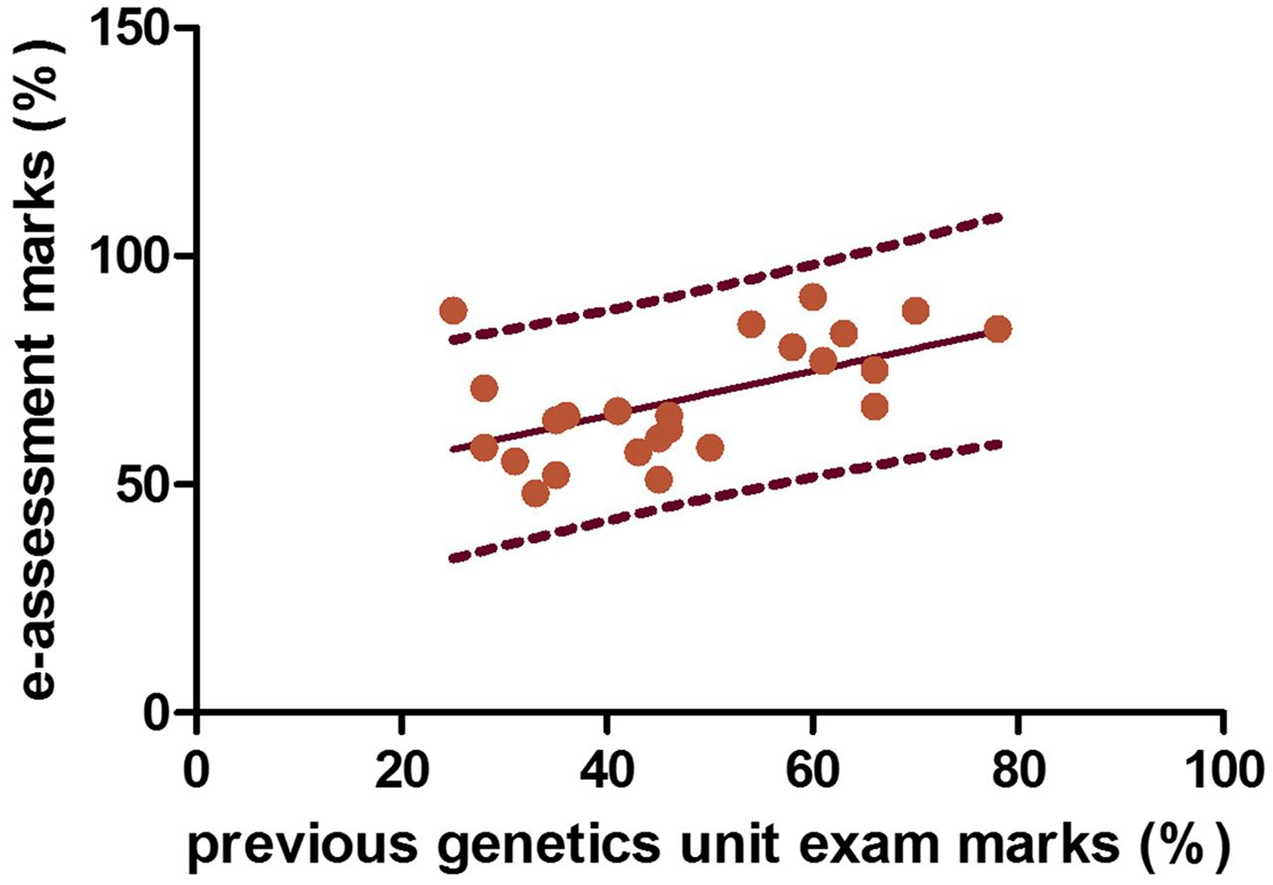
\includegraphics[width=\linewidth]{images/example-figure-g3}
\caption{Example figure from \url{http://dx.doi.org/10.1534/g3.115.017509}. Please include your figures in the 
    manuscript for the review process. You can upload figures to Overleaf via the Project menu. Upon acceptance, 
    we'll ask for your figure files to be uploaded in any of the following formats: TIFF (.tiff), JPEG (.jpg), 
    Microsoft PowerPoint (.ppt), EPS (.eps), or Adobe Illustrator (.ai).  Images should be a minimum of 
    300 dpi in resolution and 500 dpi minimum if line art images.  RGB, CMYK, and Grayscale are all 
    acceptable. Halftones should be high contrast with sharp detail, because some loss of detail and 
    contrast is inevitable in the production process. Figures should be 10-20 cm in width and 1-25 cm 
    in height. Graph axes must be exactly perpendicular and all lines of equal density.  Label 
    multiple figure parts with A, B, etc. in bolded type, and use Arrows and numbers to draw attention 
    to areas you want to highlight. Legends should start with a brief title and should be a 
    self-contained description of the content of the figure that provides enough detail to fully 
    understand the data presented. All conventional symbols used to indicate figure data points are 
    available for typesetting; unconventional symbols should not be used. Italicize all mathematical 
    variables (both in the figure legend and figure) , genotypes, and additional symbols that 
    are normally italicized.  
}%
\label{fig:spectrum}
\end{figure}

\subsection*{Sample Video}

Figure \ref{video:spectrum} shows how to include a video in your manuscript.

\begin{figure}[htbp]
\renewcommand{\familydefault}{\sfdefault}\normalfont
\centering
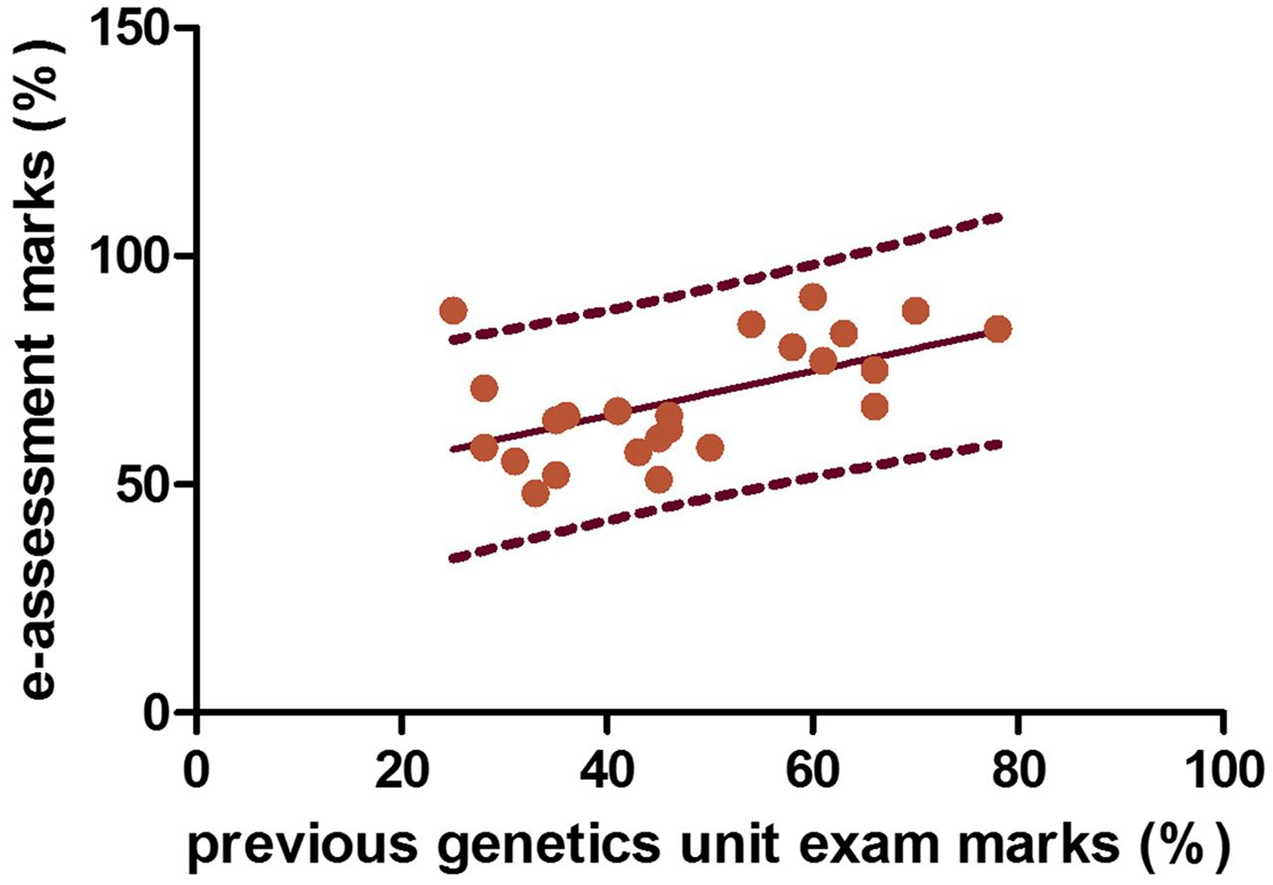
\includegraphics[width=\linewidth]{images/example-figure-g3}
\caption{Example movie (the figure file above is used as a placeholder for this example). G3 supports video and movie 
         files that can be linked from any portion of the article - including the abstract. Acceptable formats include 
         .asf, avi, .wav, and all types of Windows Media files.   
}%

\label{video:spectrum}
\end{figure}


\subsection*{Sample Table}

Table \ref{tab:shape-functions} shows an example table. Avoid shading, color type, line drawings, graphics, or 
                                other illustrations within tables. Use tables for data only; present drawings, graphics, 
                                and illustrations as separate figures. Histograms should not be used to present data 
                                that can be captured easily in text or small tables, as they take up much more space.  

Tables numbers are given in Arabic numerals. Tables should not be numbered 1A, 1B, etc., but if necessary, 
interior parts of the table can be labeled A, B, etc. for easy reference in the text.  


\begin{table*}[htbp]
\renewcommand{\familydefault}{\sfdefault}\normalfont
\centering
\caption{\bf Students and their grades}
\begin{tableminipage}{\textwidth}
\begin{tabularx}{\textwidth}{XXXX}
\hline
\header Student & Grade\footnote{This is an example of a footnote in a table. Lowercase, superscript italic letters (a, b, c, etc.) are used by default. You can also use *, **, and *** to indicate conventional levels of statistical significance, explained below the table.} & Rank & Notes \\
\hline
Alice & 82\% & 1 & Performed very well.\\
Bob & 65\% & 3 & Not up to his usual standard.\\
Charlie & 73\% & 2 & A good attempt.\\
\hline
\end{tabularx}
  \label{tab:shape-functions}
\end{tableminipage}
\end{table*}

\section*{Sample Equation}

Let $X_1, X_2, \ldots, X_n$ be a sequence of independent and identically distributed random variables with $\text{E}[X_i] = \mu$ and $\text{Var}[X_i] = \sigma^2 < \infty$, and let
\begin{equation}
S_n = \frac{X_1 + X_2 + \cdots + X_n}{n}
      = \frac{1}{n}\sum_{i}^{n} X_i
\label{eq:refname1}
\end{equation}
denote their mean. Then as $n$ approaches infinity, the random variables $\sqrt{n}(S_n - \mu)$ converge in distribution to a normal $\mathcal{N}(0, \sigma^2)$.

\bibliography{bibliography}

\end{document}
